\section{Requirements}
First, the team modeled the requirements through the use of KAOS models\cite{b2}. By building the KAOS models, the team could describe the problem to be solved and the constraint it must be fulfilled by any solution provider. Moreover, using the KAOS models, the team could remove or add new requirements easily with new changes. To gather requirements, there were various means but an efficient way was to reuse requirement patterns that are universal to software application. We specified the goals starting with the generic pattern of requirements and used it on new cases to guide the refinement of requirements.

\begin{figure*}
\centerline{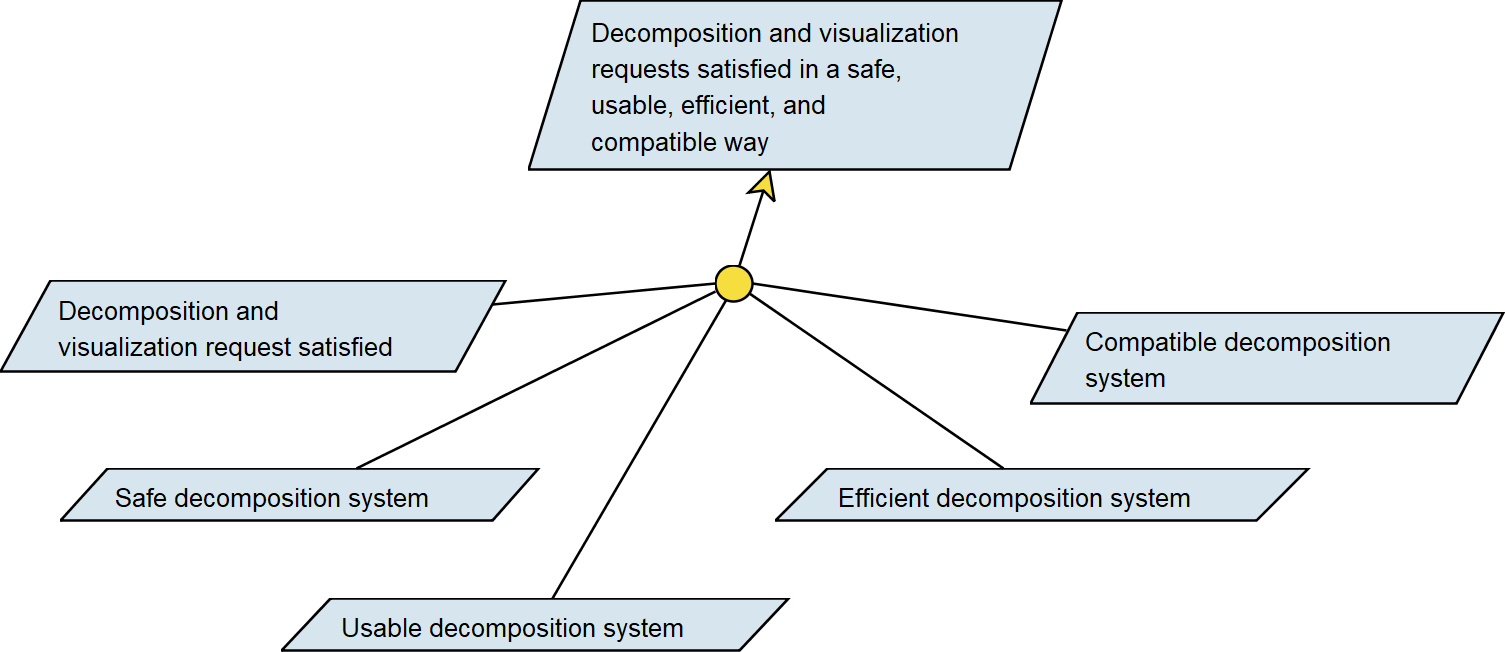
\includegraphics[width=\textwidth,height=\textheight,keepaspectratio]{./figure/GoalsNFR1.png}}
\caption{Goal: “Decomposition requests satisfied in a secure, usable, efficient, compatible, and reliable way”.}
\end{figure*}

The tactic that we used here is case-driven decomposition. We specified the subgoals that enumerate all the cases that must be covered to fulfill our main goal. The subgoals covered all the functional and nonfunctional that we wanted to include in our system. From the generic pattern, the goals that our application want to achieve are:

\begin{itemize}
	\item Decomposition and visualization request satisfied
	\item Safe decomposition system
	\item Usable decomposition system
	\item Efficient decomposition system
	\item Compatible decomposition system
\end{itemize}

Continuing with generic patterns, we reused the goal generic pattern for “Safe System”, “Usable System”, “Efficient System”, and “Compatible System”. From these models, we generated the nonfunctional requirements for our system.

\begin{center}
\begin{table}
\caption{Non-functional requirements}
\begin{tabular}{ |c|c| } 
\hline
\multicolumn{1}{|c|}{\textbf{ID}} & \multicolumn{1}{c|}{\textbf{Description}} \\
\hline
NFR1 & Show resources about Agile development \\
\hline
NFR2 & Follow Agile development process \\
\hline
NFR3 & Have presets for user without domain expertise \\
\hline
NFR4 & Show notification about decomposition status \\
\hline
NFR5 & Do not store information on third-party database \\
\hline
NFR6 & Only query Jira the information that is needed \\
\hline
NFR7 & Software is secure \\
\hline
NFR8 & Retain original sentences in epics with minimal modification \\
\hline
NFR9 & The response time for AI processing is less than five seconds \\
\hline
NFR10 & The response time for visualization is less than two seconds \\
\hline
NFR11 & Visualization only generate important relationships \\
\hline
NFR12 & Available on Atlassian Marketplace \\
\hline
NFR13 & Available on Atlassian Partner Marketplace \\
\hline
\end{tabular}
\end{table}
\end{center}

\begin{figure*}
\centerline{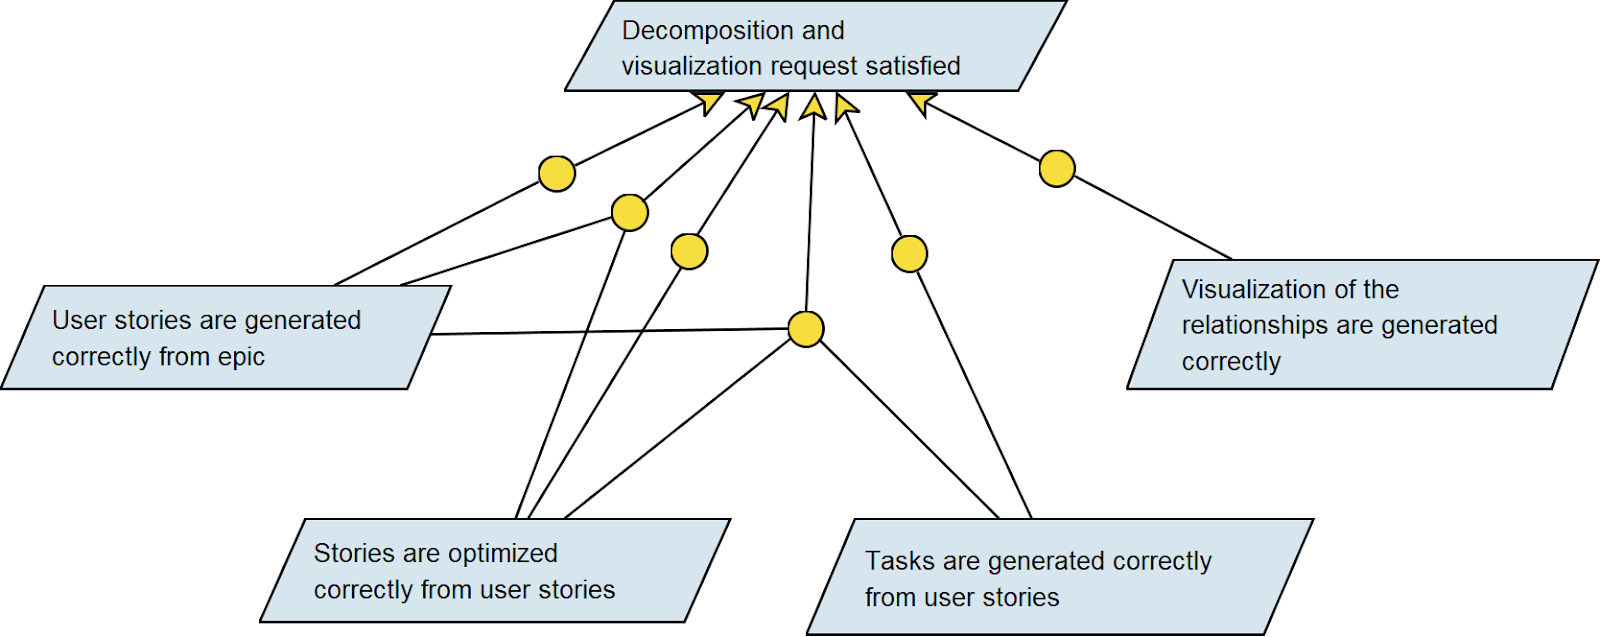
\includegraphics[width=\textwidth,height=\textheight,keepaspectratio]{./figure/GoalsNFR2.png}}
\caption{Goal: “Decomposition request and visualization satisfied”.}
\end{figure*}

Next, we broke down the “decomposition request and visualizations satisfied” goal into subgoals correlated to the main functionalities that the project proposal included. The subgoals for functional requirements are: 

\begin{itemize}
	\item User stories are generated correctly from epic
	\item Stories are optimized correctly from user stories
	\item Tasks are generated correctly from user stories
	\item Visualization of the relationships are generated correctly
\end{itemize}

The next step is to generate the requirements from all the subgoals. Each subgoal from the “Decomposition request and visualization satisfied” goal has its own KAOS model. From these models, we generated the functional requirements for our system as shown in the following table.

\begin{center}
\begin{table}
\caption{Functional requirements}
\begin{tabular}{ |c|c| } 
\hline
\multicolumn{1}{|c|}{\textbf{ID}} & \multicolumn{1}{c|}{\textbf{Description}} \\
\hline
FR1 & Clustering works correctly \\
\hline
FR2 & Allow user to select and discard generated issue \\
\hline
FR3 & Can process a variety of input type \\
\hline
FR4 & User stories extraction works correctly \\
\hline
FR5 & Retain user stories if those are small enough \\
\hline
FR6 & Sentence building works correctly \\
\hline
FR7 & Show the explicit relationship between issues as a tree \\
\hline
FR8 & Show the implicit relationship of developers to the issues as clusters \\
\hline
FR9 & Allow user to show and edit relationship \\
\hline
FR10 & Show a customizable type and depth to relationship between issues \\
\hline
FR11 & The graph should render as the object is selected \\
\hline
\end{tabular}
\end{table}
\end{center}